\section{Current Results}
\label{sec:results}
\begin{table*}[t]\centering\small
\caption{Fashion-Gen test results (\%; 9 brands, 5 era years; 95\% product-bootstrap intervals in brackets). ``Both'' = brand and era both correct.}\label{tab:fashiongen}
\begin{tabular}{lccccc}\toprule
Model & Brand acc. & Brand F1 & Era acc. & Era F1 & Both \\\midrule
Majority class & 28.9 & --- & 31.7 & --- & --- \\
8$\times$8 thumbnail, linear probe & 34.4 & 19.1 & 41.4 & 38.2 & --- \\\midrule
CLIP ViT-B/16, linear probe & 56.9 \ci{53.7}{59.8} & 53.3 & 69.7 \ci{66.9}{72.2} & 69.5 & 40.7 \\
CLIP ViT-B/16, $k$-NN & 53.4 \ci{50.4}{56.3} & 46.7 & 55.7 \ci{52.8}{58.6} & 54.3 & 34.4 \\
DINOv2 ViT-S/14, linear probe & 52.5 \ci{49.4}{55.4} & 48.2 & 64.3 \ci{61.6}{66.9} & 64.5 & 35.1 \\
DINOv2 ViT-S/14, $k$-NN & 49.9 \ci{47.1}{52.7} & 42.9 & 50.6 \ci{47.8}{53.5} & 49.2 & 29.5 \\
ResNet-50, linear probe & 45.3 \ci{42.5}{48.1} & 41.0 & 53.2 \ci{50.5}{55.9} & 52.6 & 25.7 \\
ResNet-50, $k$-NN & 44.7 \ci{41.8}{47.6} & 34.2 & 41.9 \ci{39.3}{44.5} & 39.8 & 21.0 \\\midrule
CLIP ViT-B/16 fine-tuned (strong aug.) & 65.3 \ci{62.2}{68.2} & 62.8 & 81.3 \ci{78.5}{84.0} & 81.5 & 55.0 \\
\bottomrule\end{tabular}\end{table*}


\begin{figure}[t]
\centering
\includegraphics[width=\columnwidth]{figures/samples.pdf}
\caption{Test images from the proxy datasets: Fashion-Gen catalog photos (CDG, Margiela, Undercover,
Yohji), second-hand brand-label close-ups, and Europeana catwalk looks (1990s/2000s/2010s).}
\label{fig:samples}
\end{figure}

\paragraph{Frozen features (Table~\ref{tab:fashiongen}).}
On Fashion-Gen, CLIP is the strongest frozen encoder for both brand (56.9\% vs.\ a 28.9\% majority
baseline) and era (69.7\% vs.\ 31.7\%), ahead of DINOv2 and ResNet-50, and the linear probe beats
$k$-NN for every encoder and task. Era errors are concentrated on adjacent years, and era accuracy
stays high within the five brands that span all five years (CDG 75\%, Helmut Lang 71\%, Margiela
69\%, Raf Simons 71\%, Yohji 70\%), so the era head is not simply reading off the brand.

\begin{figure*}[t]
\centering
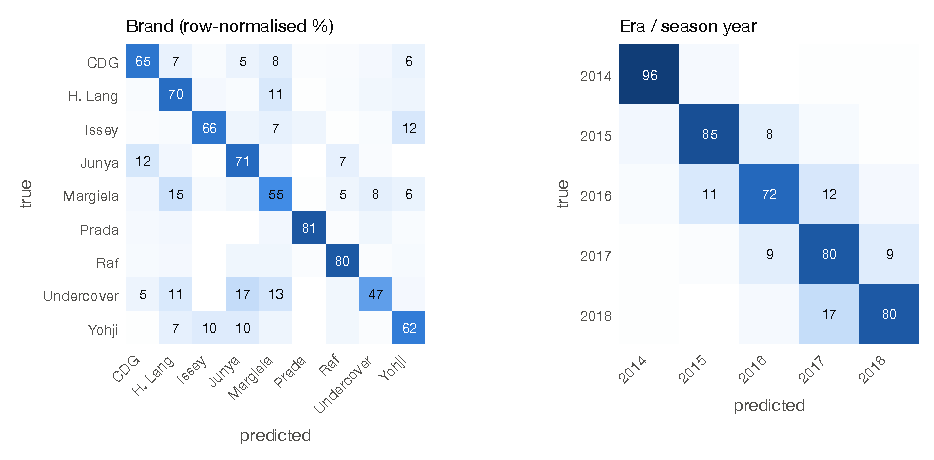
\includegraphics[width=0.84\textwidth]{figures/confusion_fashiongen.pdf}
\caption{Fashion-Gen test confusion matrices of the fine-tuned CLIP model (rows = true class,
row-normalized \%). Era errors fall mostly on adjacent years.}
\label{fig:confusion}
\end{figure*}

\paragraph{Fine-tuning (Table~\ref{tab:fashiongen}, Fig.~\ref{fig:confusion}).}
Fine-tuning CLIP with phone-photo augmentation raises Fashion-Gen brand accuracy from 56.9\% to
65.3\% and era accuracy from 69.7\% to 81.3\%, and gets both right for 55.0\% of test images (40.7\%
for the frozen probe). The confusions are plausible: Undercover, the weakest class, is mistaken for
Junya Watanabe and Margiela; Junya (a Comme des Gar\c{c}ons-group label) for CDG; Margiela and
Helmut Lang for each other; and Issey Miyake for Yohji Yamamoto. 83\% of era errors fall on
adjacent years.

\paragraph{Label photos and runway decades (Table~\ref{tab:other}).}
The label-photo proxy separates the encoders most clearly: a CLIP linear probe identifies the brand
from a label close-up 78.0\% of the time (11 brands), versus 35.2\% for DINOv2 and 27.1\% for
ResNet-50. The gap is consistent with CLIP's image--text pretraining making its features sensitive to printed
text, much more so than purely visual pretraining (not yet tested directly); it is the strongest
argument for CLIP as our backbone, since the real input is a label. Fine-tuning CLIP with phone-photo augmentation raises this to 84.6\%.
Many label photos are upside down or sideways, so our first OCR
experiment runs EasyOCR with rotated text boxes and matches brand names within single text lines
(short names must match a whole word; ties abstain). With the match threshold tuned on validation,
OCR answers for 34.0\% of test labels and is never wrong on them; trusting it when it answers and
the image model otherwise lifts the CLIP probe from 78.0\% to 82.2\% and the fine-tuned model from
84.6\% to 87.0\%. OCR and the image model are complementary: where OCR answers, the image model
alone still errs 12\% of the time, and stylized woven logos need the image model. For archive labels, OCR will additionally target printed date and
product codes (Sec.~\ref{sec:eras}).
On Europeana runway photos (10 designers, show-grouped splits), CLIP reaches 63.7\% brand and
81.8\% decade accuracy (majority 45.3\%); with only 76 test shows the intervals are wide. The 1990s
class holds only late-1990s shows (1997--99) of four houses, and an 8$\times$8 thumbnail alone already
predicts the decade 60.6\% of the time, so part of the decade signal is photographic.

\begin{figure*}[t]
\centering
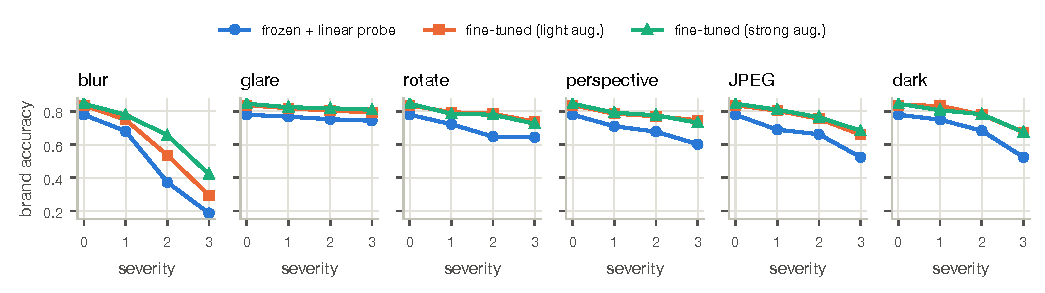
\includegraphics[width=\textwidth]{figures/robustness_secondhand_labels.pdf}
\caption{Label-photo brand accuracy under six test-time corruptions at severities 1--3 (0 = clean),
CLIP ViT-B/16. Severity-averaged values: Table~\ref{tab:robustness_secondhand_labels}.}
\label{fig:robustness}
\end{figure*}
\begin{table}[t]\centering\small
\caption{Second-hand labels brand accuracy (\%) under test-time corruptions, averaged over severities 1--3 (CLIP ViT-B/16; FT = fine-tuned with light or strong augmentation).}\label{tab:robustness_secondhand_labels}
\begin{tabular}{lccc}\toprule
Condition & Frozen probe & FT, light & FT, strong \\\midrule
Clean & 78.0 & 83.7 & 84.6 \\\midrule
Blur & 41.4 & 52.7 & 61.9 \\
Glare & 75.5 & 80.6 & 81.8 \\
Rotate & 67.2 & 77.3 & 76.4 \\
Perspective & 66.4 & 76.8 & 76.7 \\
JPEG & 62.6 & 74.0 & 75.3 \\
Dark & 65.3 & 76.3 & 75.5 \\
\midrule Mean of corruptions & 63.0 & 73.0 & 74.6 \\
\bottomrule\end{tabular}\end{table}


\paragraph{Robustness to phone-photo conditions (Fig.~\ref{fig:robustness}).}
On label photos, fine-tuning helps under every corruption: averaged over the six corruptions and
three severities, accuracy rises from 63.0\% (frozen probe) to 74.6\% (fine-tuned with phone-photo
augmentation). The augmentation's clearest benefit is against blur (61.9\% vs.\ 52.7\% with light
augmentation); for the other corruptions the two fine-tuned models are within about one point,
which is within noise on 332 test images. Blur remains the hardest condition, so the final app should ask
for a retake when a photo is blurry.
On Fashion-Gen the gap is starker: averaged over the corruptions, the fine-tuned model keeps 60.4\%
brand and 77.3\% era accuracy (65.3\% / 81.3\% clean), while the frozen probe falls to 36.2\% and
36.9\% (era majority 31.7\%), consistent with its era signal resting partly on fragile photographic
cues.

\begin{table}[t]\centering\footnotesize
\caption{Test accuracy (\%) on the label-photo and runway proxies.}\label{tab:other}
\setlength{\tabcolsep}{2pt}\begin{tabular}{@{}lcc@{}}\toprule
Model & Brand & Era \\\midrule
\multicolumn{3}{l}{\emph{Second-hand labels} (11 brands)} \\
\quad Majority class & 12.7 & --- \\
\quad 8$\times$8 thumbnail probe & 12.7 & --- \\
\quad CLIP probe & 78.0 \ci{73.5}{82.5} & --- \\
\quad DINOv2 probe & 35.2 \ci{30.4}{40.4} & --- \\
\quad ResNet-50 probe & 27.1 \ci{22.6}{31.9} & --- \\
\quad CLIP fine-tuned (light aug.) & 83.7 \ci{79.8}{87.7} & --- \\
\quad CLIP fine-tuned (strong aug.) & 84.6 \ci{80.7}{88.6} & --- \\
\quad OCR alone (answers 34.0\%) & 34.0 & --- \\
\quad OCR, else CLIP probe & 82.2 \ci{77.7}{86.1} & --- \\
\quad OCR, else fine-tuned (light aug.) & 86.1 \ci{82.2}{89.8} & --- \\
\quad OCR, else fine-tuned (strong aug.) & 87.0 \ci{83.1}{90.7} & --- \\
\multicolumn{3}{l}{\emph{Europeana runway} (10 brands, 3 eras)} \\
\quad Majority class & 12.6 & 45.3 \\
\quad 8$\times$8 thumbnail probe & 33.6 & 60.6 \\
\quad CLIP probe & 63.7 \ci{56.2}{70.4} & 81.8 \ci{76.5}{86.7} \\
\quad DINOv2 probe & 60.7 \ci{52.1}{68.7} & 71.7 \ci{64.5}{78.4} \\
\quad ResNet-50 probe & 51.6 \ci{44.3}{58.4} & 65.9 \ci{59.8}{71.7} \\
\bottomrule\end{tabular}\end{table}


\paragraph{Value estimation.}
Retrieval works: the prices of the 10 most similar catalog items predict an item's retail price
with a median error of 31.2\% (Spearman $\rho=0.70$), against 43.5\% for a global median and 41.7\%
for the median price of the item's \emph{true} brand; within-brand prices vary too much for the
brand alone to help. Ridge regression on log price is comparable (32.5\%), but retrieval also
returns the comparable items, which is what a reseller wants to see.

\paragraph{Shortcut checks.}
A linear probe on an 8$\times$8-pixel thumbnail, or on the colour statistics of the image border
alone, predicts the Fashion-Gen year with 41.4\% / 37.0\% accuracy (majority 31.7\%), so photography
style carries some era signal; CLIP's 69.7\% is far beyond that, but shoot-level cues (models,
styling) that a grouped split cannot remove may still contribute, so era must ultimately be judged
on label photos. On the label photos the thumbnail probe
is at chance (12.7\% vs.\ a 12.7\% majority) and the border-colour probe close to it (14.8\%), so
the sorting-station backgrounds give little away.
